\documentclass[a4paper,12pt]{article}
\usepackage{caption}
\usepackage{subcaption}
\usepackage{graphicx}
\graphicspath{ {img/} }
\usepackage{fancyhdr}
\pagestyle{fancy}
\lhead{tqvj24}
\chead{}
\rhead{Image Processing Assignment}
\lfoot{tqvj24}

\begin{document}

\section*{Discussion and detail of system design and choices made}
\subsection*{System Design}
I wrote this script using Python 3.5.2, and OpenCv 3.1.0, to match the versions available on the DUDE PCs in the School.
Operation of the script is done via key presses, and output of the program is both visual in the main window, as well as various images being saved to disk, in the img\_out/ directory.
The main window displays one file ID at a time, with the top row being the w1 channel, and the bottom being w2. These are labelled, and labelling can be toggled by pressing the l key.
Full list of commands:
\begin{itemize}
    \item n - next image
    \item b - previous image
    \item l - toggle labels
    \item s - save the currently displayed w1 and w2 processed images
    \item x - exit
\end{itemize}
There are also boolean settings toward the top of the script, to allow for automatic saving of various images. \\
Processing of images is done in steps, with each step being a standalone method. All methods are documented and commented. The processing steps are as follows:
\begin{enumerate}
    \item Isolate and Compare
    \begin{enumerate}
        \item\textbf{Isolate} the worms from the background and border.
        \item\textbf{Compare} the isolated worms against the provided ground truth.
    \end{enumerate}

    \item Individualise and Save each worm
    \begin{enumerate}
        \item Run the \textbf{watershed} algorithm to mark worms with unique colours.
        \item Save each individual worm to disk, under img\_out/separated/ directory. This sub-step also prints how many worms have been counted in the given image.
    \end{enumerate}

    \item Label each worm either dead or alive
    \begin{enumerate}
        \item Find the rotated bound box of each contour, and classify dead or alive depending on the width/height ratio of said box.
    \end{enumerate}
\end{enumerate}
Examples of what the above steps produce can be found under later sections. All images shown here are of A01 w2, to clearly show the changes.

\subsection*{Choices Made}
As the images are saved as 16 bit but only really using 12 bits, when reading as 8 bit images the 4 most significant bits were lost, and the image was very dark (Figure a), and so I read in the images as 16 bit, right shifted by 4 bits, and then converted to 8 bit. This ignores the 4 least significant bits, in favour of the 4 most significant bits. This results in a much more usable and bright image (Figure b).\\
\begin{figure}[ht!]
    \centering
    \begin{subfigure}{0.5\textwidth}
        \centering
        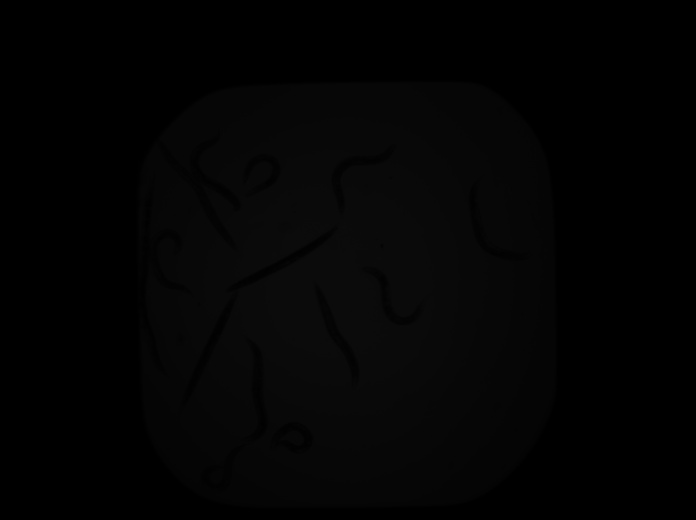
\includegraphics[width=0.8\textwidth]{A01_step0_unshifted.jpg}
        \caption{Loaded as 8 bit}
    \end{subfigure}%
    \begin{subfigure}{0.5\textwidth}
        \centering
        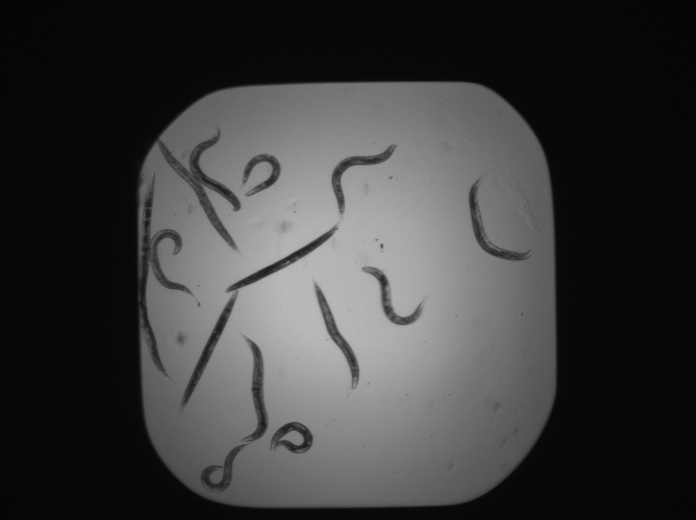
\includegraphics[width=0.8\textwidth]{A01_step0.jpg}
        \caption{Loaded as 16 bit and shifted}
    \end{subfigure}
\end{figure}
\\
I then had to ensure the image was of reasonable brightness, and I found OpenCV's adaptive threshold to be much more effective than it's histogram equalisation, and the possibility to go straight to a binary image proved useful.
\\\\
The next choice I made was border removal for w2. My initial attempt found all contours, and assumed the largest was the border, filling this in black to remove it. This worked for most images, although big worm clusters were occassionally larger than the border in area, and so were removed instead. I instead settled on dilating a flood fill that started from the point (0, 0). This meant that it would surround the border, and slowly grow over it. Experimenting with the values given to this function resulted in very good border removal.
\\\\
When comparing my binary images to the provided binary images, I decided to simply subtract one from the other, so that the resulting image's white pixels were representative of the error of my conversion. While this always resulted in high percentage values due to large empty spaces, and a big border surrounding the plate itself, other methods seemed to always provide no measure of how big or small their result actually was, they were just numbers without context.
\\
To detect which worms were dead, and which were alive, I initially tried using contours, which could be checked by a method called isContourConvex, as this would indiciate whether the worm was curved or not. However, this method was inconsistent, and unreliable in actually providing a boolean return, so I changed to finding the bounding box of the contour, and checking whether it is long and thin, or approximately square.

\section*{Evidence of the success of system in performing the specified task}
\subsection*{Processing Steps}
The loaded image, before any of the major processing steps, is shown below as Figure 1.
\\\\
Step 1, which isolated the worms from the background and border, produced Figure 2.
\\\\
Step 2, which isolated individual worms, produced Figure 3 where worms are all outlined in red, and Figure 4 which has each worm coloured a different shade of grey.
\\\\
Step 3, which drew boxes around worms, and coloured them green if considered alive, red if considered dead, produced Figure 5, the final image which is shown on screen during runtime.

\begin{figure}[ht!]
    \centering
    \begin{subfigure}{0.5\textwidth}
        \centering
        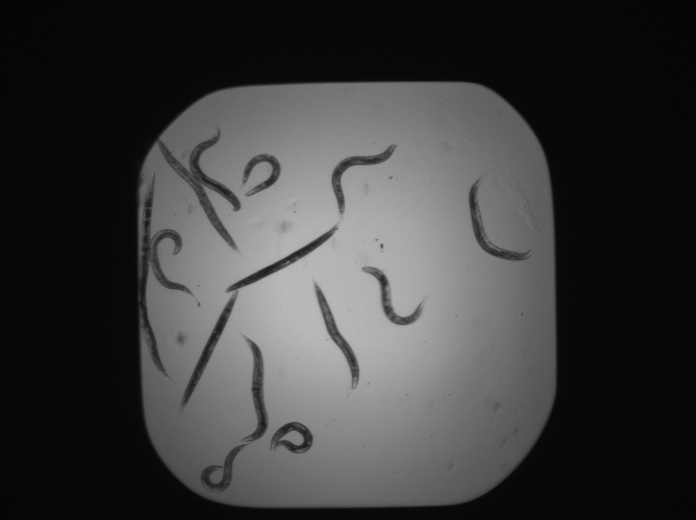
\includegraphics[width=0.8\textwidth]{A01_step0.jpg}
        \captionsetup{labelformat=empty}
        \caption{Figure 1}
    \end{subfigure}%
    \begin{subfigure}{0.5\textwidth}
        \centering
        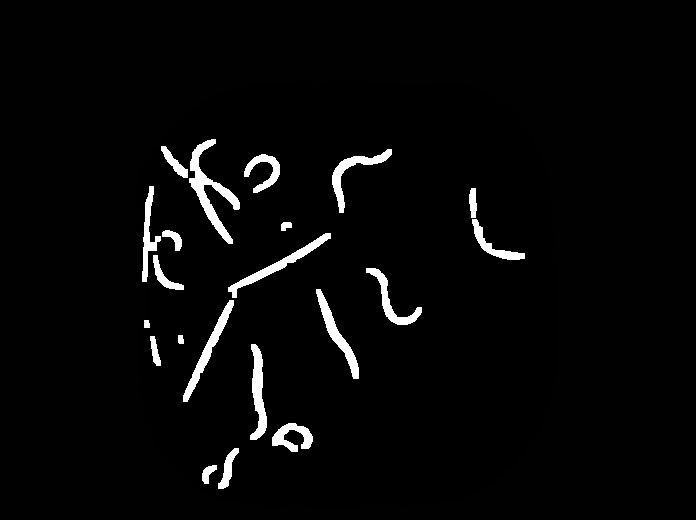
\includegraphics[width=0.8\textwidth]{A01_step1.jpg}
        \captionsetup{labelformat=empty}
        \caption{Figure 2}
    \end{subfigure}
    \begin{subfigure}{0.5\textwidth}
        \centering
        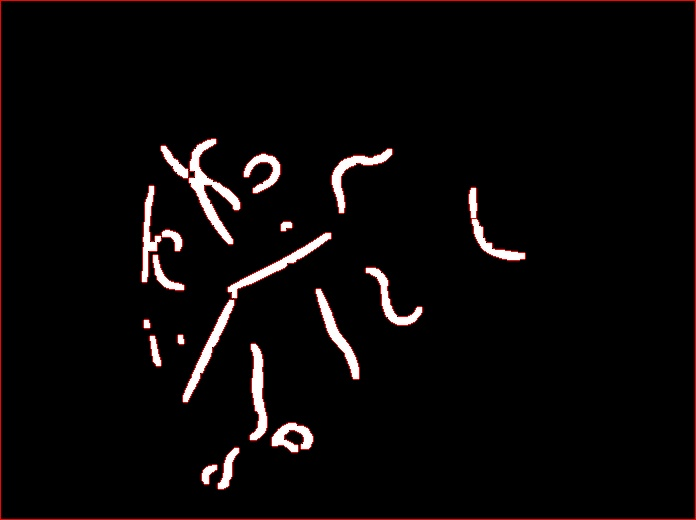
\includegraphics[width=0.8\textwidth]{A01_step2.jpg}
        \captionsetup{labelformat=empty}
        \caption{Figure 3}
    \end{subfigure}%
    \begin{subfigure}{0.5\textwidth}
        \centering
        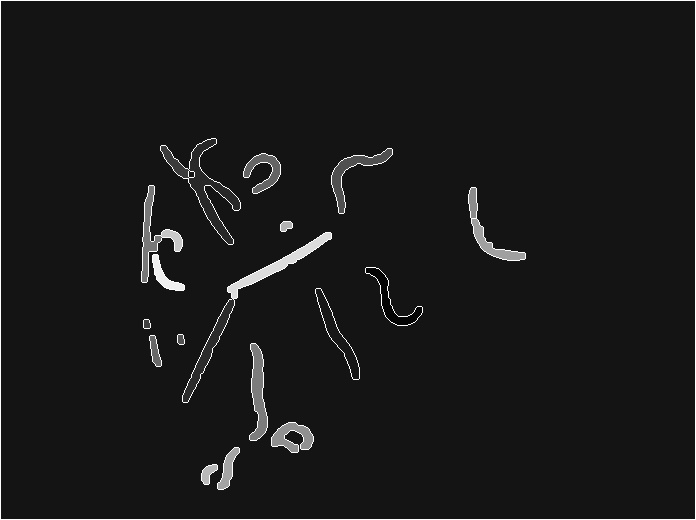
\includegraphics[width=0.8\textwidth]{A01_step2_markers.jpg}
        \captionsetup{labelformat=empty}
        \caption{Figure 4}
    \end{subfigure}
    \centering
    \begin{subfigure}{0.8\textwidth}
        \centering
        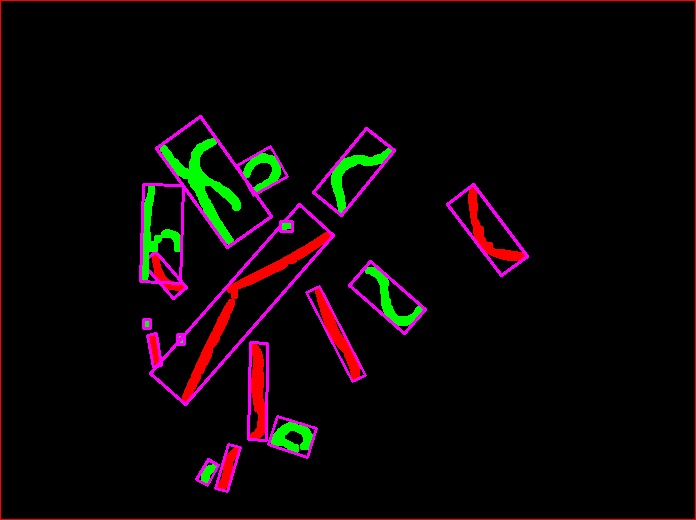
\includegraphics[width=0.8\textwidth]{A01_step3.jpg}
        \captionsetup{labelformat=empty}
        \caption{Figure 5}
    \end{subfigure}
\end{figure}

\end{document}
